\documentclass[runningheads]{llncs}
\usepackage[colorlinks=true,urlcolor=black,linkcolor=cyan,citecolor=cyan]{hyperref}
\usepackage[hyphenbreaks]{breakurl}

\pagenumbering{arabic}

\usepackage{url}
\usepackage{times}
\usepackage{graphicx}
\usepackage{amsmath}
\usepackage{latexsym}
\usepackage{enumerate}
\usepackage{color}
\usepackage{booktabs}
\usepackage{pifont}
\usepackage[nocompress]{cite}

\usepackage{dcolumn}
\newcolumntype{d}[1]{D{.}{.}{#1}}
\newcolumntype{.}{D{.}{.}{-1}}

\newcommand{\be}{\begin{equation}}
\newcommand{\ee}{\end{equation}}
\newcommand{\ba}{\begin{eqnarray}}
\newcommand{\ea}{\end{eqnarray}}



\newcommand{\urlBiBTeX}[1]{\url{#1}} %%% needed for URL to print nice

\begin{document}

\title{{\Large Facing the St-Petersburg Paradox:} \\{\large How Security Researchers Make Money with Bug Bounty Markets?}}%\thanks{This research was supported in part by the National Science Foundation through award CCF-0424422 (TRUST - Team for Research in Ubiquitous Secure Technology).}}

\author{Anonymous submission}
\date{}

\maketitle

\begin{abstract}
Bug bounty programs offer a modern platform for organizations to crowdsource their software security and for security researchers to be fairly rewarded for the vulnerabilities they find. Little is known however on the incentives set by bug bounty programs: How they drive new bug submissions, and how they improve security through the progressive exhaustion of discoverable vulnerabilities. Here, we recognize that bug bounty programs create tensions for organizations running them on the one hand, and for security researchers on the other hand. At the level of one bug bounty program, security researchers face a sort of St-Petersburg paradox: The probability of finding additional bugs decays fast, and thus can hardly be matched with a sufficient increase of monetary rewards. Furthermore, bug bounty program managers have an incentive to gather the largest possible crowd to ensure a larger pool of expertise, which in turn increases competition among security researchers. As a result, we find that researchers have high incentives to switch to newly launched programs, for which a reserve of {\it low-hanging fruit} vulnerabilities is still available. Our results inform on the technical and economic mechanisms underlying the dynamics of contributions, and may in turn help improve the mechanism design of bug bounty programs that get increasingly adopted by cybersecurity savvy organizations.
\end{abstract}
%\mynormality{1.2}
%\newpage
\section{Introduction}
\label{sec:intro}
Software security is a hard problem, which requires automatic and human testing....\\

Crowdsourcing has become a popular way to find solutions to {\it hard problems}, such as sorting galaxies \cite{smith2013introduction}, or folding proteins \cite{khatib2011algorithm} for the sake of science, or to recognize words from books digitalized with low quality \cite{von2003captcha} and to solve big data problems \cite{narayanan2011link}. Even hard mathematical problems get addressed on open collaboration platforms \cite{gowers2009massively,cranshaw2011polymath}.\\

Finding software bugs and vulnerabilities has been one of the most long-standing challenges in computer science \cite{}, and similarly, crowdsourcing has been suggested over the last decade as a way to efficiently cope with software cybersecurity, through a number mechanisms, such as vulnerability brokerage \cite{camp2004pricing}, markets \cite{schechter2002buy} and auctions, with their presumed incentives, strengths and weaknesses \cite{ozment2004bug}.\\

Recently, however, ``bug bounty" platforms, essentially focused on crowdsourcing software vulnerabilities, have appeared and rapidly developed \cite{zhao2014exploratory,zhao2015empirical}. These online platforms offer both an infrastructure and play the role of {\it trusted third party} (TTP) between organizations (i.e., mainly Internet companies) and security researchers willing to search and submit the vulnerabilities they find.\\

As markets of some sort, as we shall describe more in details later, these platforms inform on transactions occurring between organizations and security researchers, and thus, they are thought to reveal the {\it true value} of vulnerabilities. They also provide empirical evidence on the economic behaviors of the parties involved (at least on the publicly facing parts of platform).\\

In this paper, we recognize the visionary theoretical propositions made more than 10 years ago by pioneering researchers in economics of information security \cite{schechter2002buy,ozment2004bug}, and we confront and enrich these propositions with empirical evidence.\\

In particular, we find that indeed the bug bounty platform studied here (i.e., HackerOne) works essentially as a {\bf (reverse?)} Dutch auction \cite{}. (we cannot exclude that the designers of the platform got inspired by the article published in 2005 \cite{ozment2004bug}). There are however a number of differences and refinements from the theory, which can be rationalized by business and organization contingencies. Also, our results provide a more accurate picture of challenges faced by researchers when engaging in bug bounties (i.e., the St. Petersburg paradox of bug bounty hunting), and the consolidation of monetary rewards over several bug bounty programs and how new bug bounty programs suddenly shift incentives.\\

This article is organized as follows. Related research is presented in Section \ref{sec:related}. Important features of the data set used here is detailed in Section \ref{sec:data}. We then introduce the main mechanism driving vulnerability discovery in Section \ref{sec:method}. Results are presented and discussed in respectively Sections \ref{sec:results} and \ref{sec:discussion}. We finally in conclude in Section \ref{sec:conclusion}.
\section{Related work}
\label{sec:related}

related work
\section{Data}
\label{sec:data}
The data were collected from the public part of the Hacker One website \cite{hackerOne}. From 35 public bounty programs, we collected the awards received by security researchers, with their timestamps and rewards in dollars. Since HackerOne started its platform in December 2013, new programs have been launched roughly every two months, following an essentially memoryless Poisson process ($\lambda = 57$ days, $p < 0.001$ and $R^2 > 0.99$). Figure \ref{timeline}{\bf A} shows the timeline of the 9 most active programs with at least 90 (rewarded) bug discoveries as of February 15, 2016. When a new program is launched, we observe an initial peak (or within weeks after launch), which accounts for the majority of discoveries, suggesting a ``windfall" effect, attracting already registered security researchers on the one hand, and newly enrolled researchers on the other hand {\bf (see Figure or Table \ref{xxx} for an account of contributions to bug discoveries by new and previously registered researchers)}. Following the initial surge of vulnerability discoveries, bounty awards become less frequent following a decay function with long-memory, following a robust power law decay $\sim t^{\alpha}$ with $\alpha = -0.40(4)$ ($p < 0.001$ and $R^2 = 0.79$) at the aggregate level and over all 35 bounty programs, with weekly time series of bug discoveries normalized by their initial value (see Figure \ref{timeline}{\bf B}).\\


\begin{figure}[h]
\begin{center}
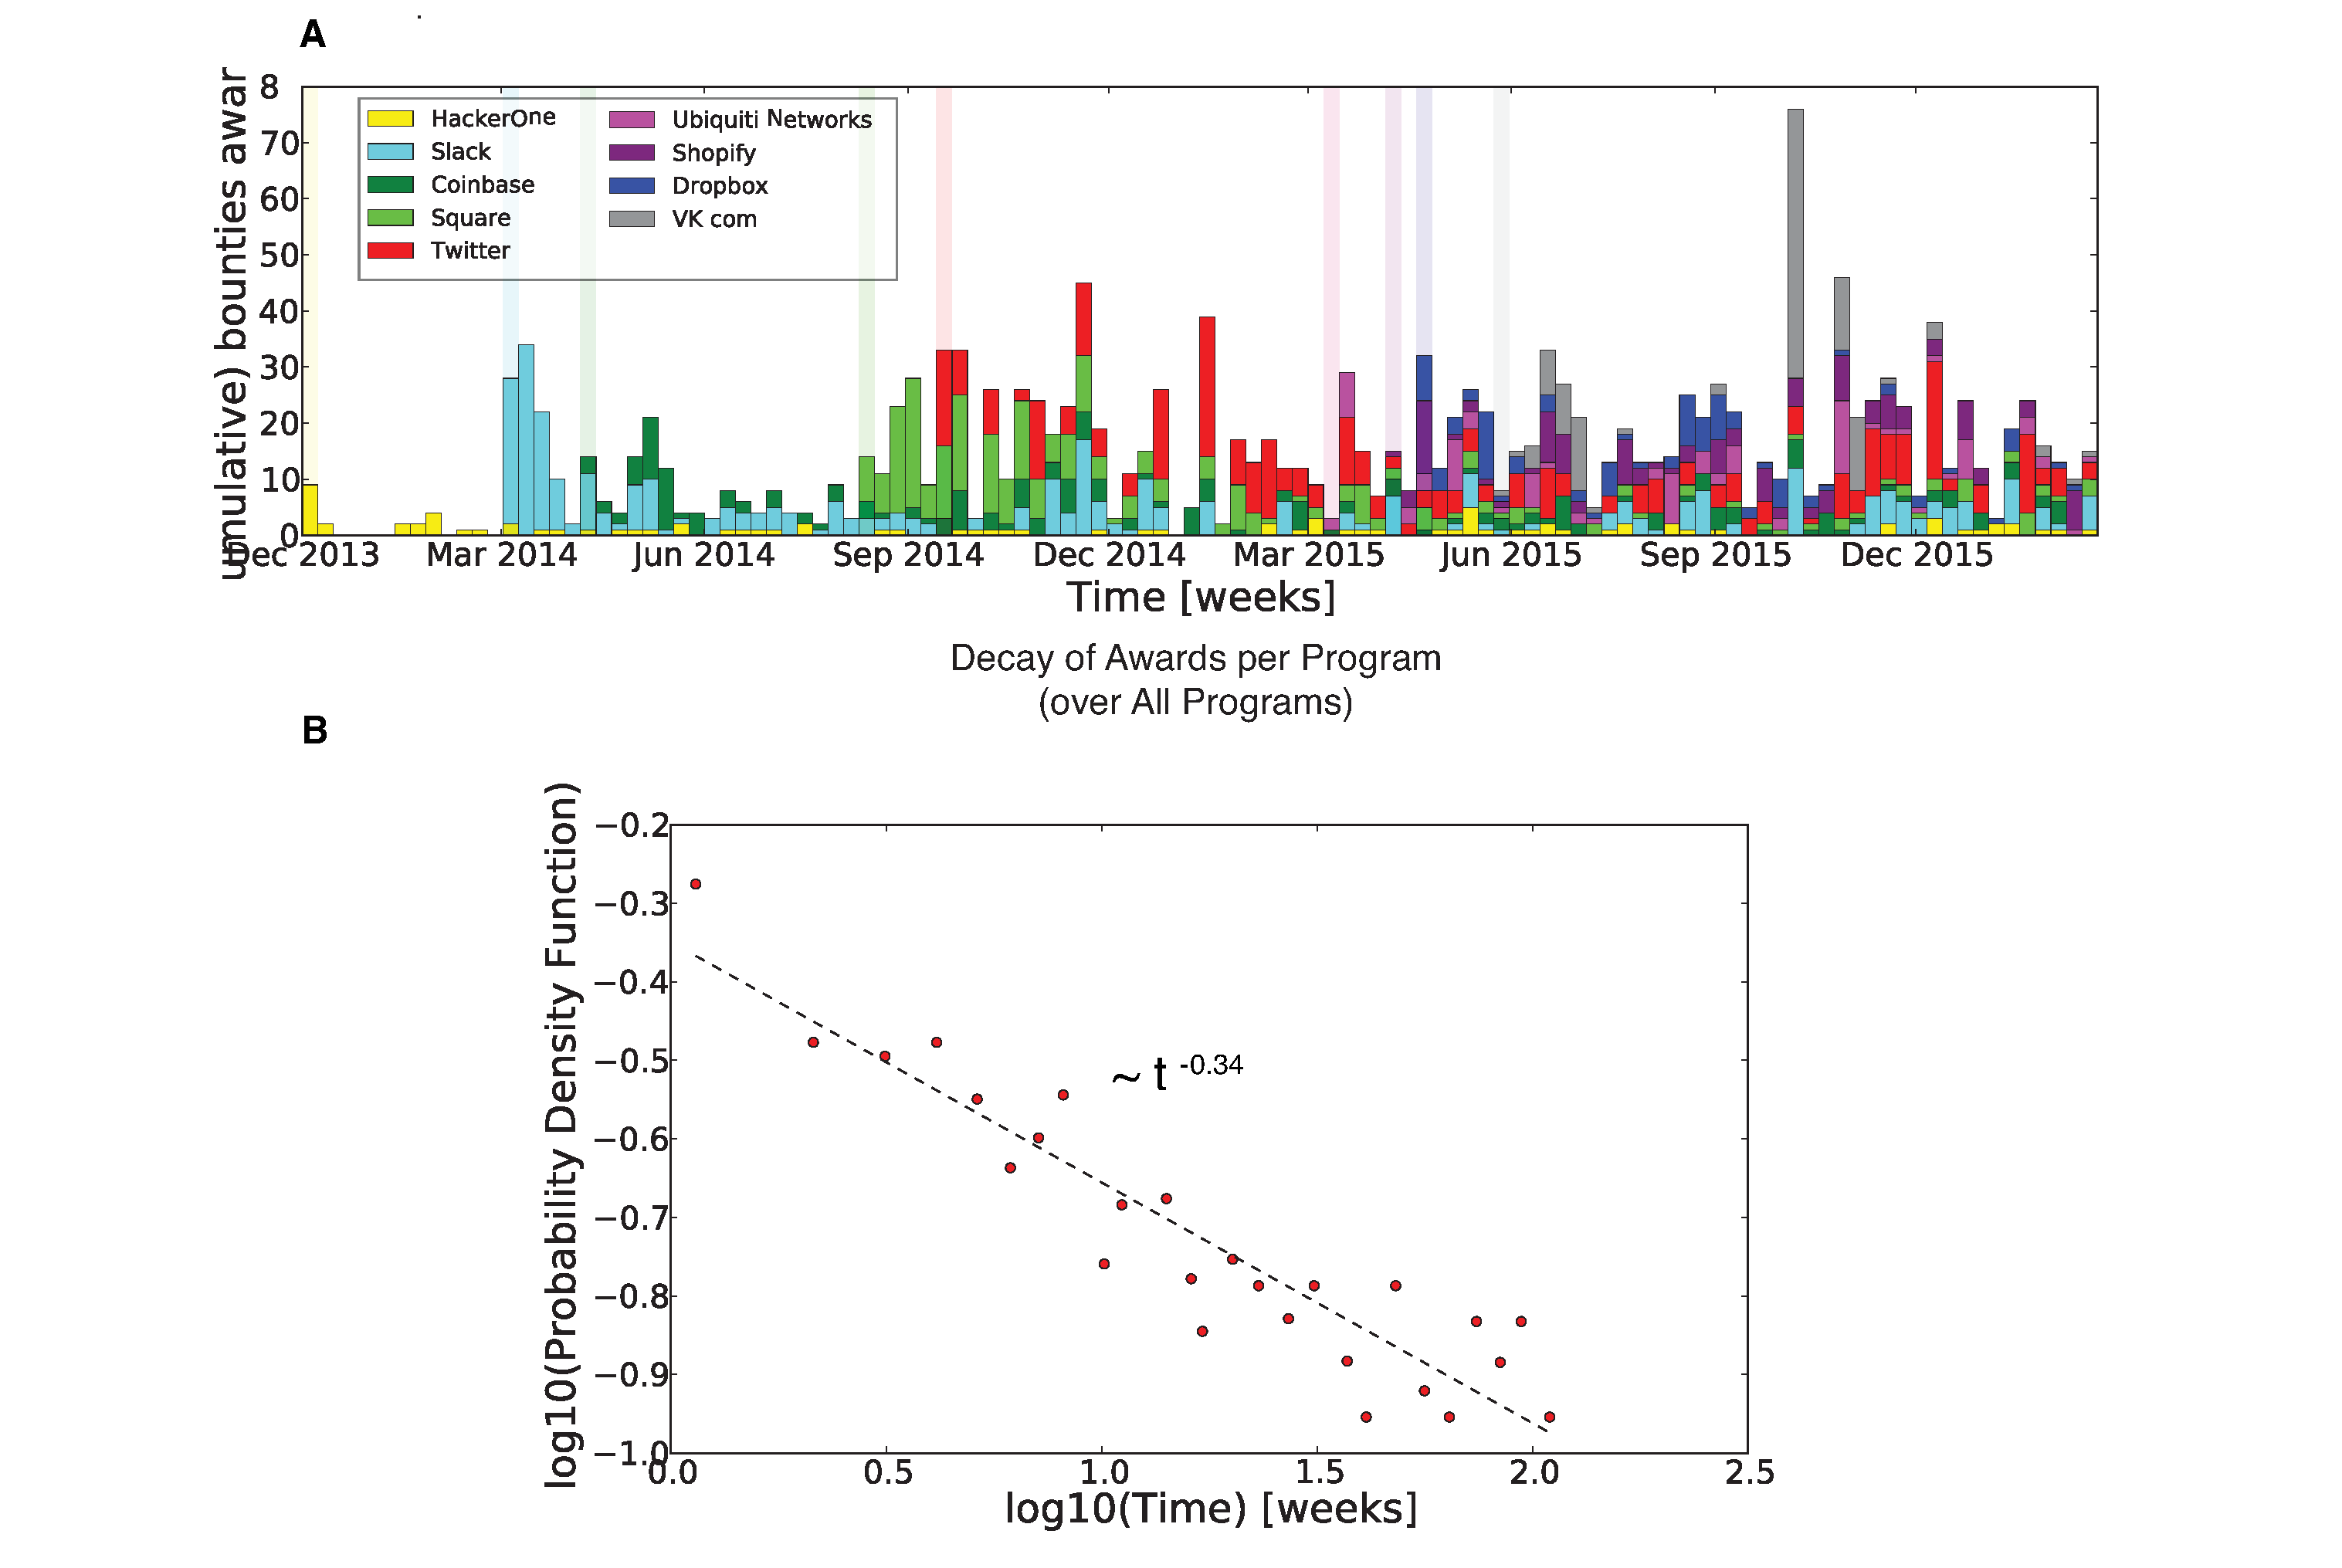
\includegraphics[width=17cm]{figures/timeline.eps}
\caption{{\bf A.} Weekly vulnerability discoveries for the 9 most active programs (with at least 90 bug discoveries as of February 15, 2016). The light colored vertical bars represent the start of the program, occurring when the first bounty is awarded. Most programs exhibit an initial shock (or shortly after the start of the program), followed by a decay of discoveries, which is characterized at the aggregate level by a long-memory process (panel {\bf B}) characterized by a power law decay $\sim t^{\alpha}$ with $\alpha = -0.40(4)$ ($p < 0.001$ and $R^2 = 0.79$) as shown on panel  (for all 35 public programs considered in this study).}
\label{timeline}
\end{center}
\end{figure}



The long-memory process of bug discovery following the launch of a bounty program we observe here, is reminiscent of human timing effects: When the program launches, it takes some time first for the researcher to be exposed (through the media) to the new program, second for the researcher to find and submit bugs, and third for the organization managing the bug bounty program to assess the quality of each submission, and assign a proper bounty reward. To account for all these delays, one may resort to priority queueing applied to humans: First, competing attention prevents immediate exposure to the news of a new program; Second, when security researchers get interested to a new program, they may still be actively searching bugs on other programs or performing other tasks, such as e.g., their regular job, leisure, family matters); Third, when subjected to a flow of bug submissions, security teams at organizations leading bounty programs assign priorities among submissions, and resolve them with human resources available at the time of submission. These delays are best rationalized by human timing contingencies, and moreover, by time as a scare, non-storable resource, and are known to generate long-memory responses of the form $\sim t^{-1.5}$ (in fully rational case) between the arrival and the execution of a task\cite{maillart2011quantification}. The observed much slower decay may result from the compound effect of multiple delays, such as those mentioned above. Since, we consider only the {\it time of discovery} as the moment when the validity of the bug submitted is acknowledged by the program manager, we are mostly blind to the human timing effects associated with the long-memory process observed on Figure \ref{timeline}{\bf B}, including when submissions are made, but don't lead to a discovery (i.e., when the value of the submission is acknowledged by a monetary reward).\\

The initial burst of discoveries, followed by a long-memory decay may also result from the increasing difficulty associated with finding new bugs for each bounty program, as the most obvious vulnerabilities get uncovered first. We thus consider a time-ordered set of bounty rewards $B_p= \{b_1,b_2,b_3,b_k, ..., b_n\}$ for each bounty program $p$, which, on average, maps into a set ordered by difficulty $\widehat{D}$, such that $\widehat{D}(b_{k+1}) > \widehat{D}(b_{k})$.\\
 
The discovery of new bugs in a bounty program is contingent to the number of active security researchers (in the program), and how many vulnerabilities each research is able to find: For a given bounty program, we shall consider the set of bounties $B_{p,r}$ associated with bugs found by researcher $r$.\\

We also investigate how the launch of a new bounty program is likely to create a new windfall effect, hence attracting researchers currently busy searching bugs in already existing bounty programs





\section{Method}

%\input{sections/analysis}
\section{Results}
\label{sec:results}

\begin{figure}
\begin{center}
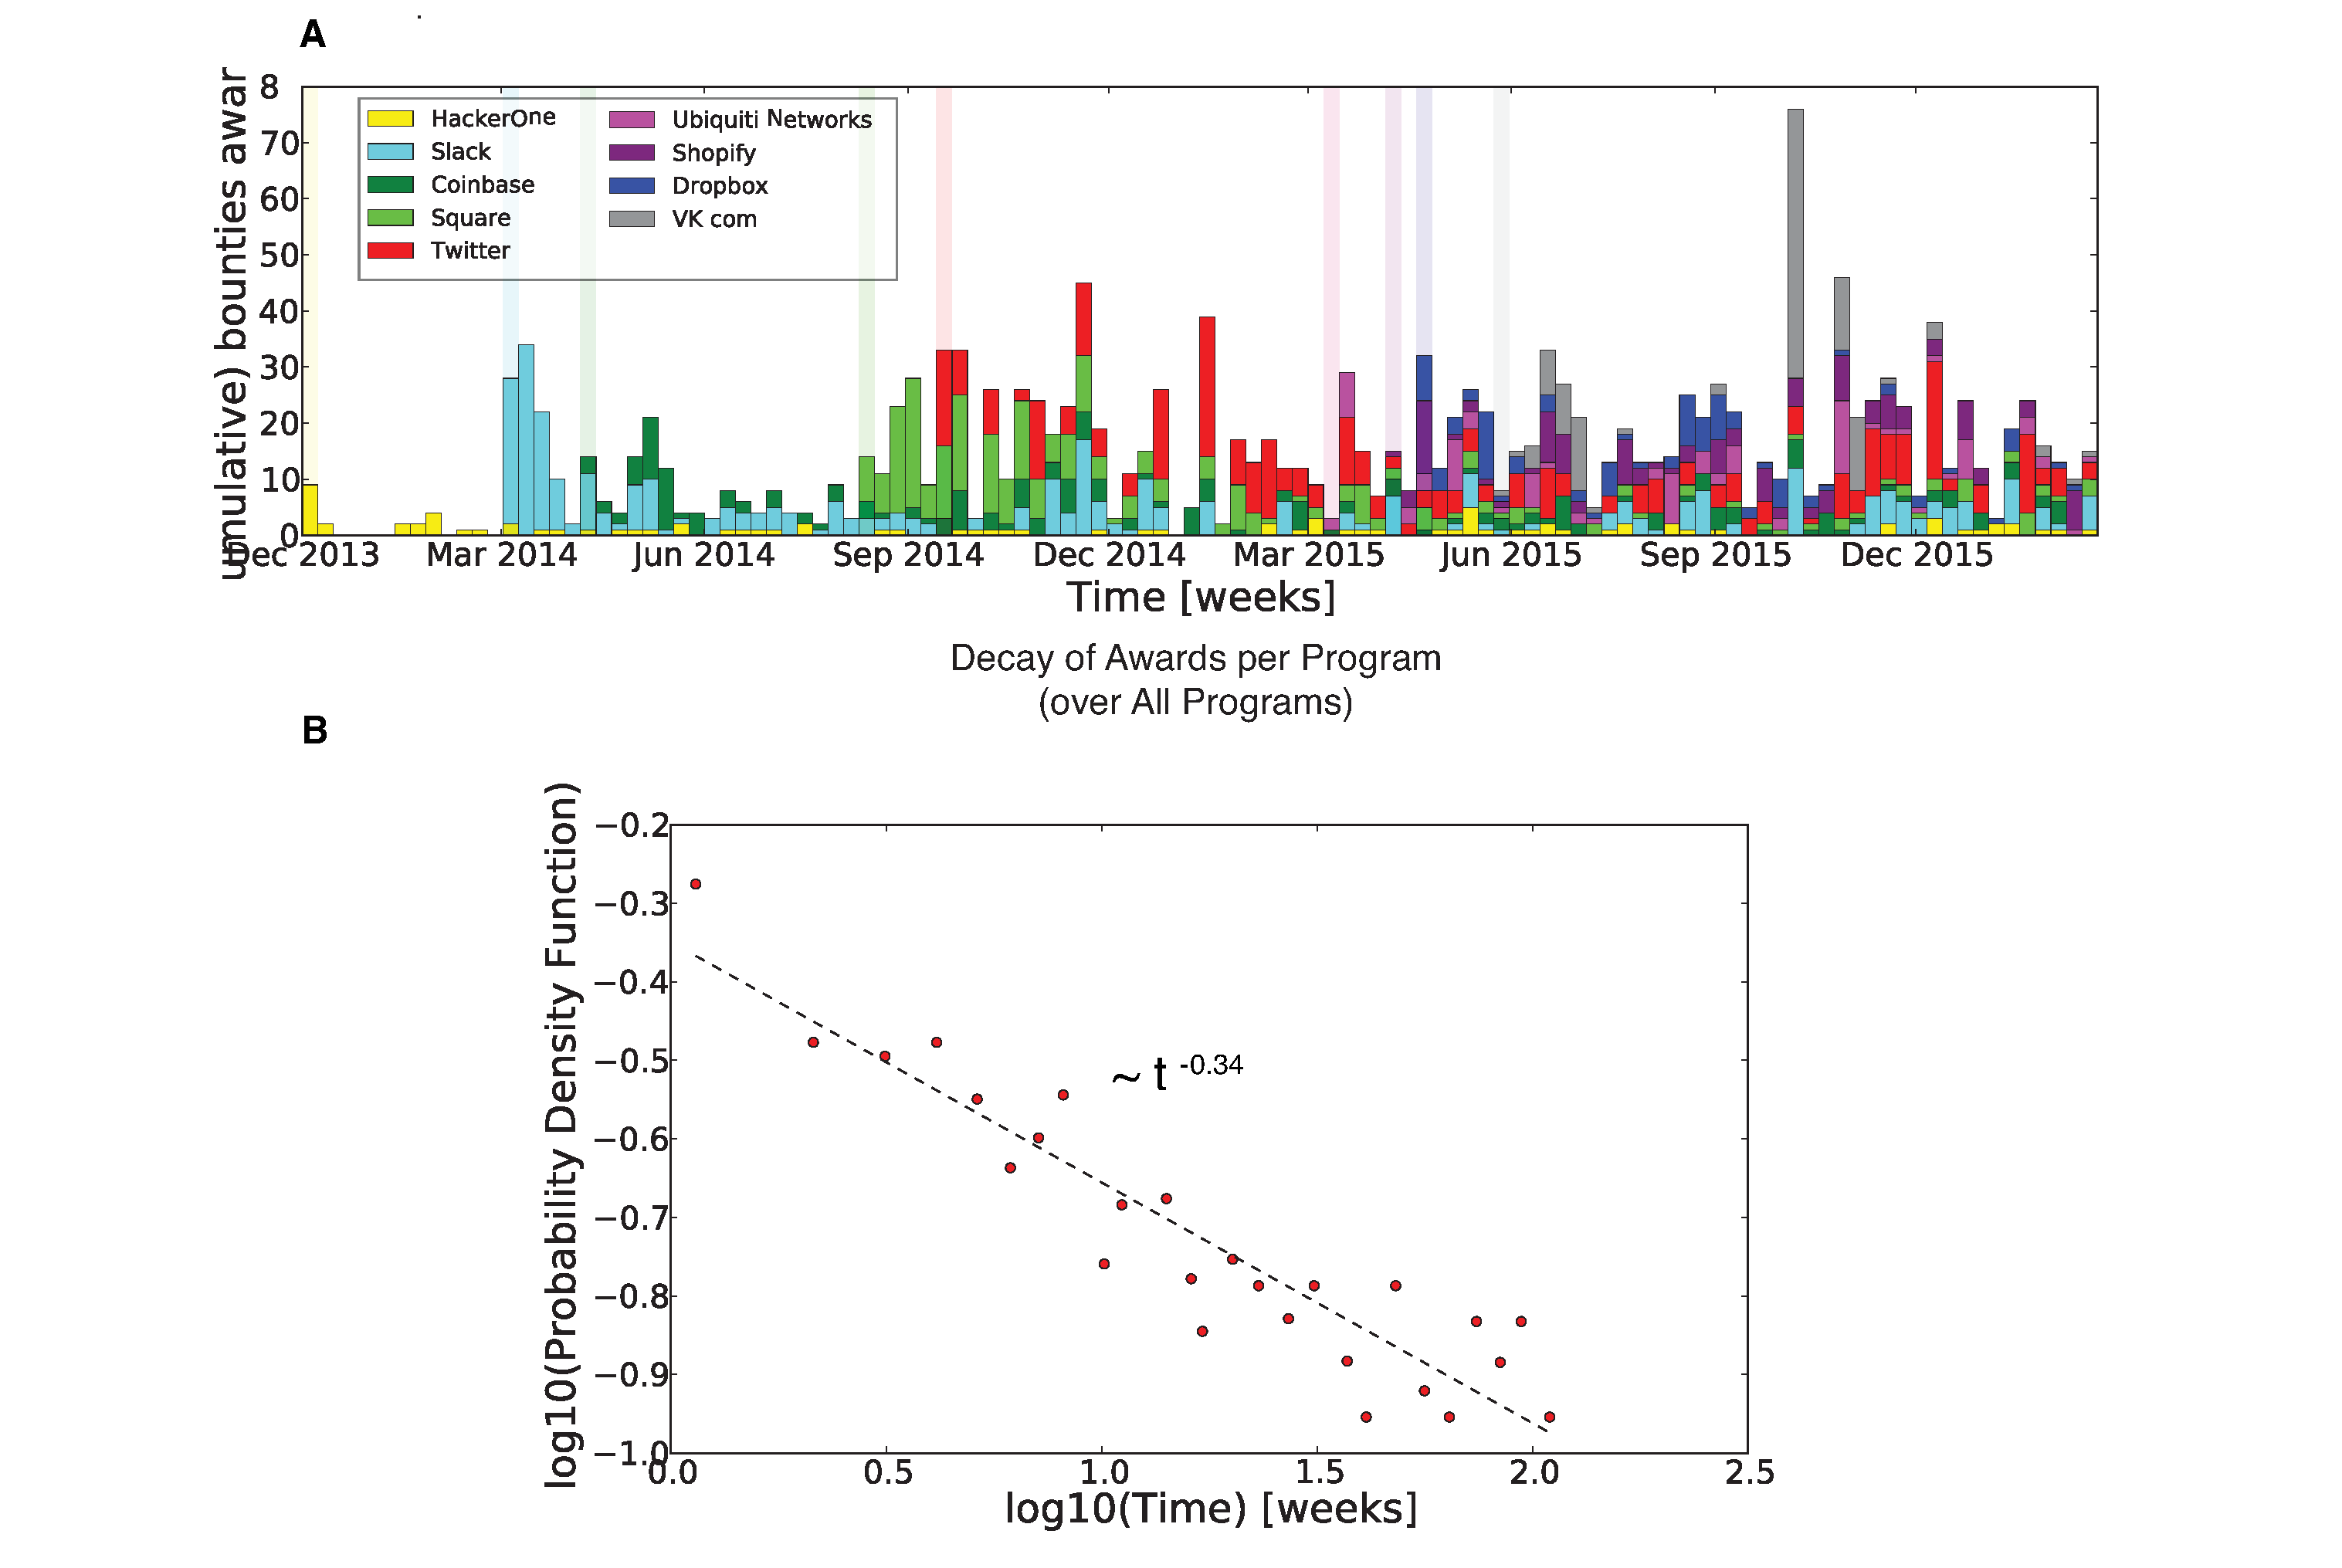
\includegraphics[width=17cm]{figures/timeline.eps}
\caption{}
\label{ }
\end{center}
\end{figure}

\begin{figure}
\begin{center}
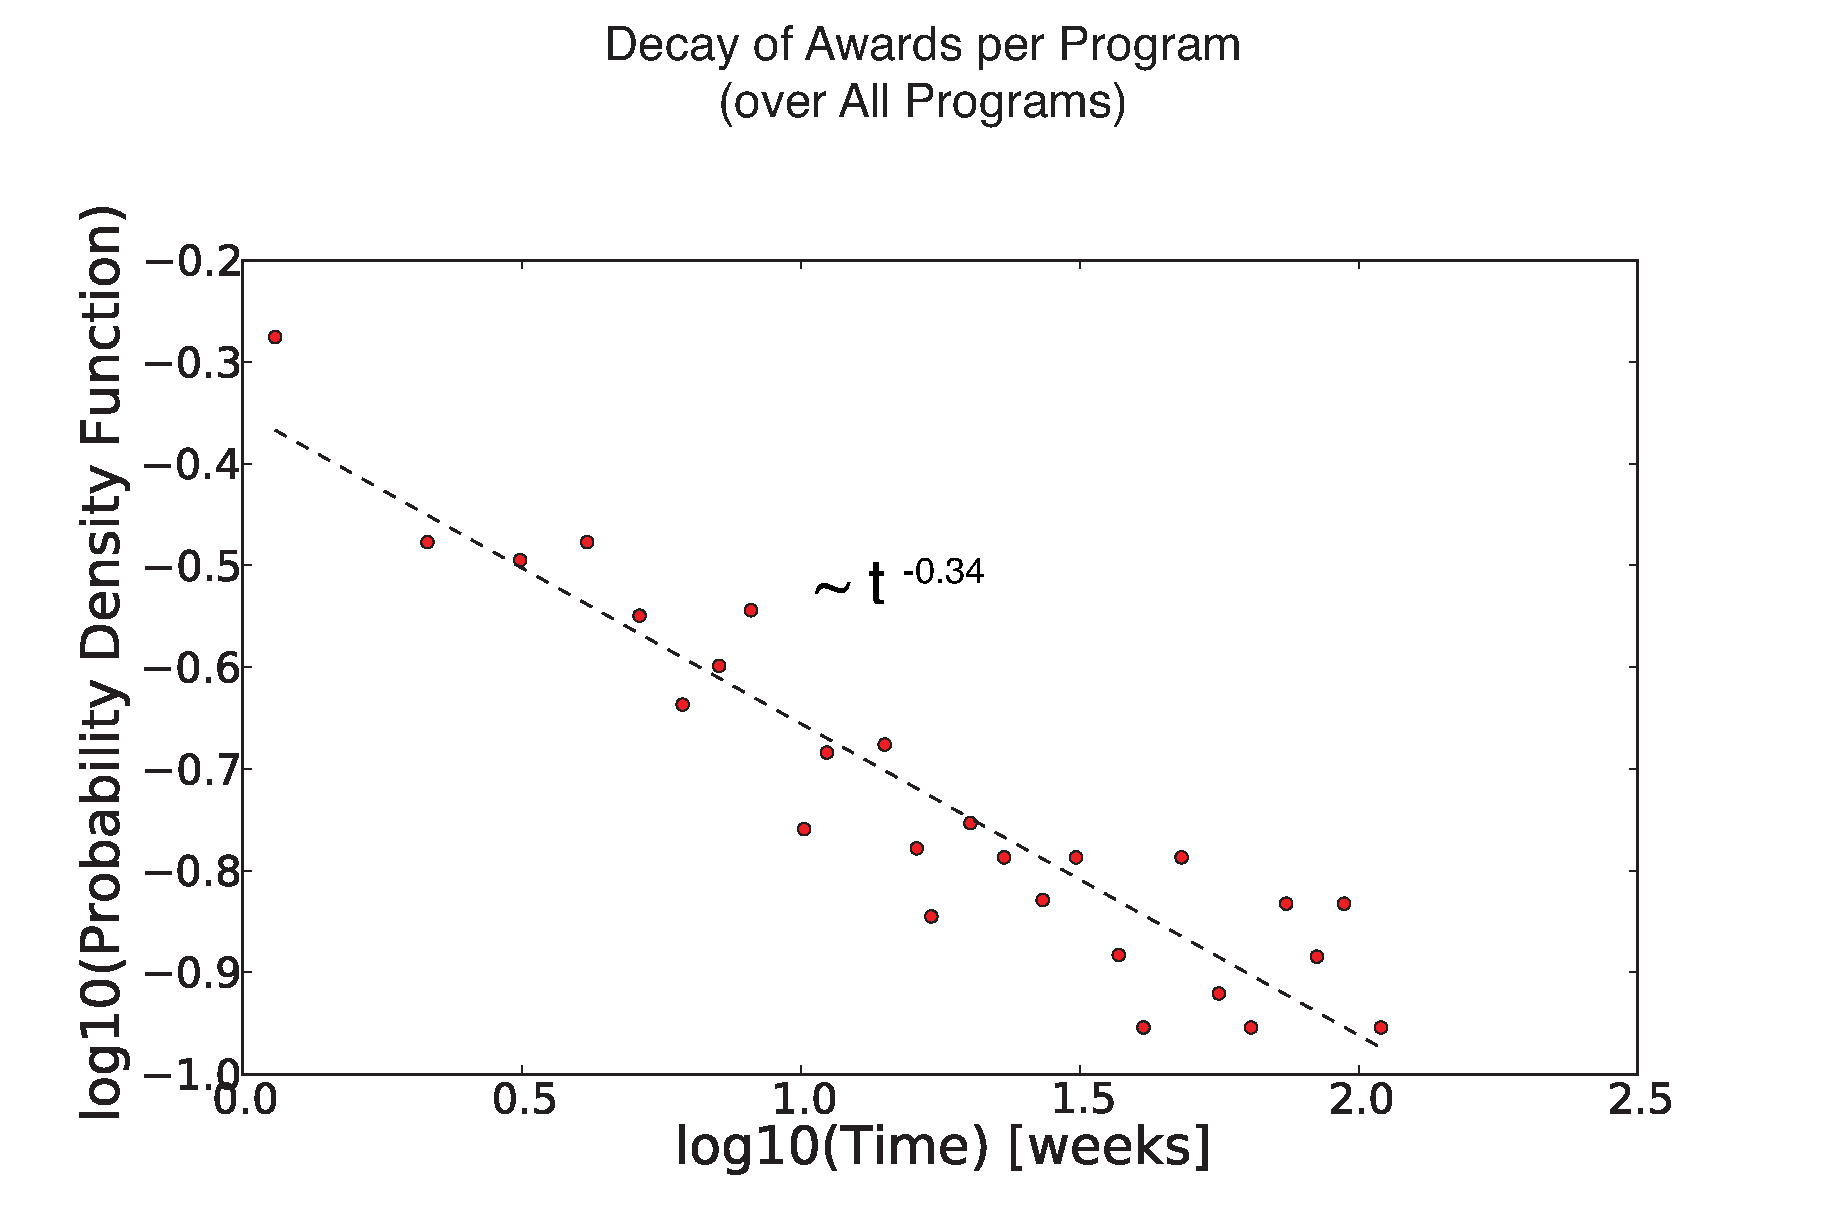
\includegraphics[width=10cm]{figures/decay.eps}
\caption{}
\label{ }
\end{center}
\end{figure}


\begin{figure}
\begin{center}
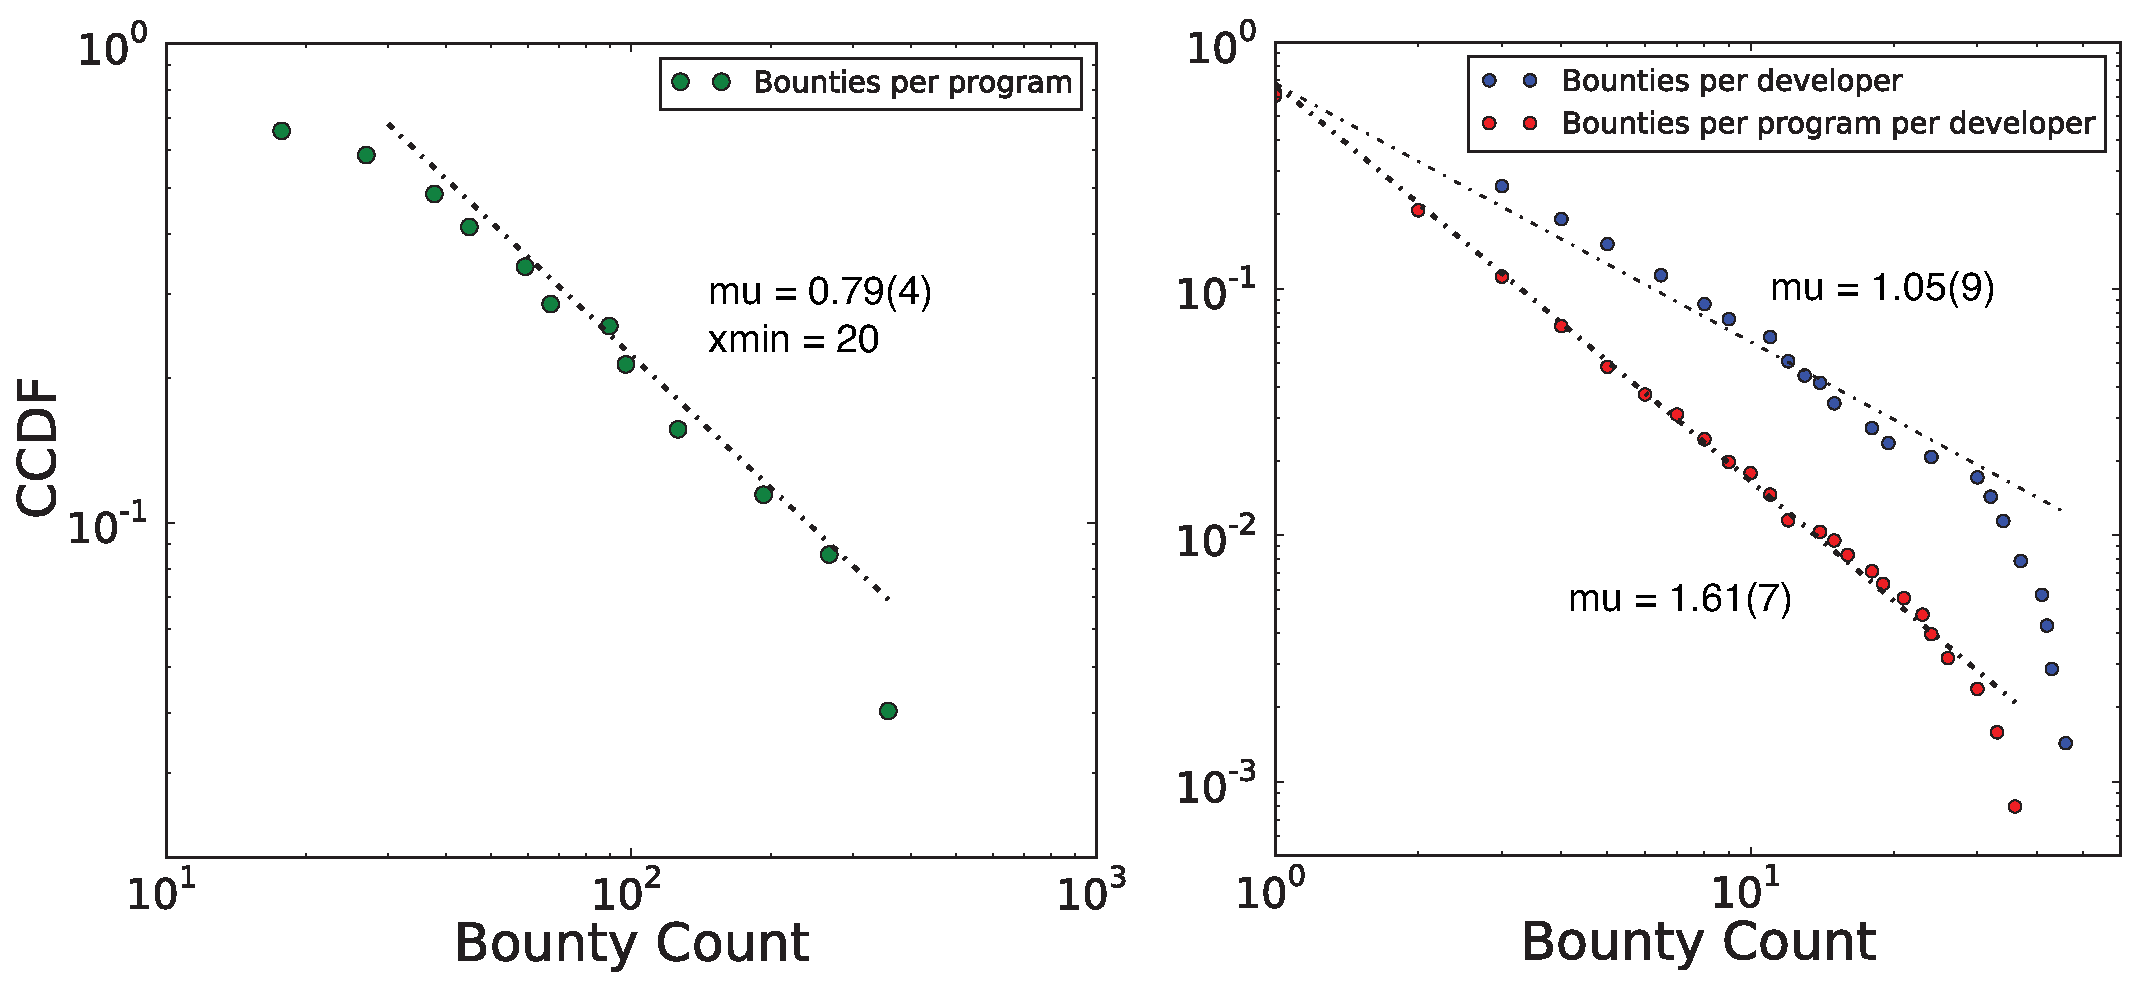
\includegraphics[width=12cm]{figures/CCDF_count_Bounties.eps}
\caption{}
\label{ }
\end{center}
\end{figure}


\begin{figure}
\begin{center}
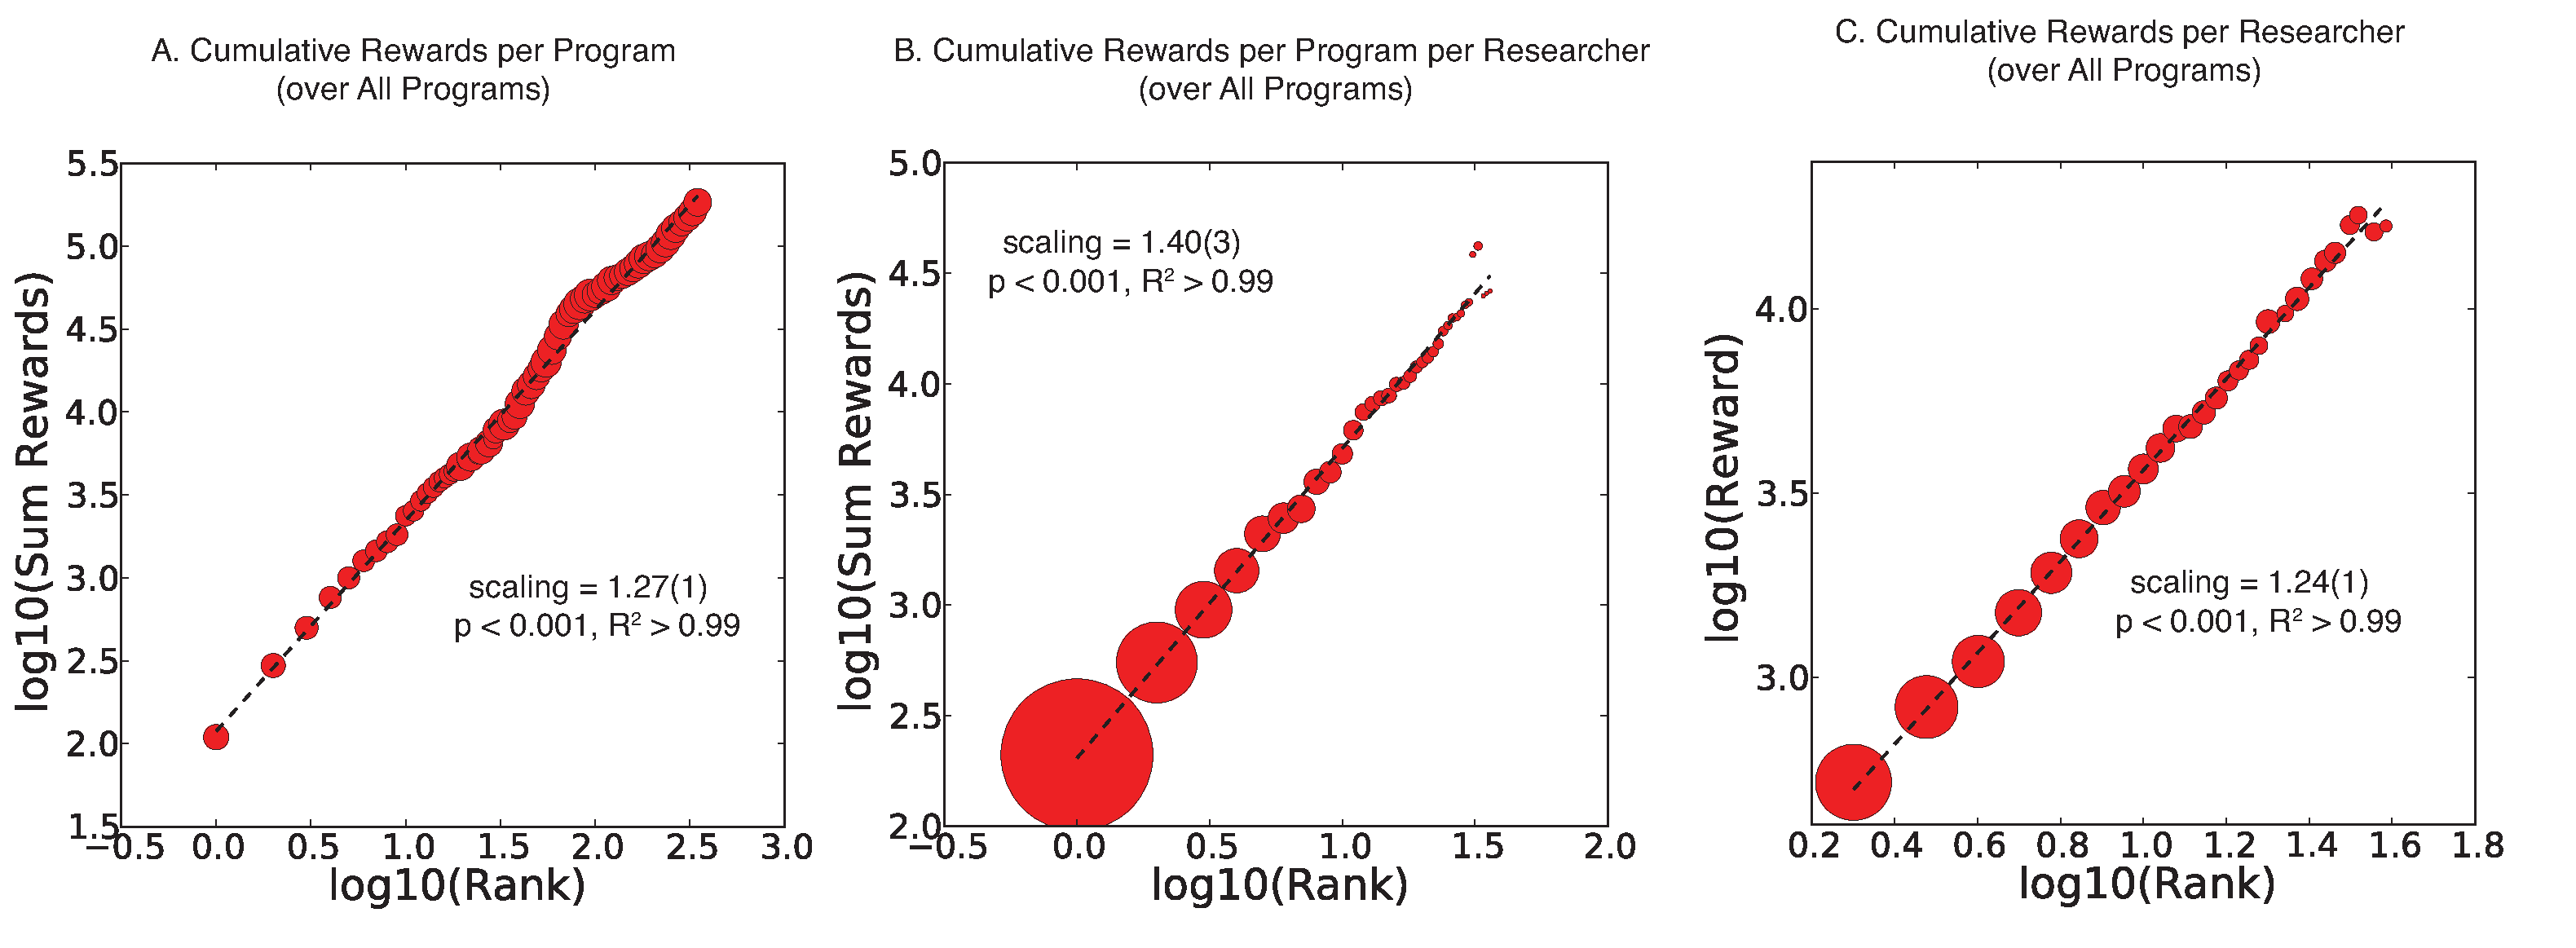
\includegraphics[width=16cm]{figures/scalings.eps}
\caption{}
\label{ }
\end{center}
\end{figure}

\section{Discussion}
\label{sec:discussion}
Finding bugs in software code is one of the oldest and toughest problems in software engineering. While algorithm based approaches have been developed over the years, human verification has remained a prime way to debugging and vulnerability hunting. Moreover, the idea of getting ``enough eyeballs" to inspect the code has been a cornerstone argument for the open source software movement \cite{raymond1999cathedral} along with the full-disclosure argument, as well as for vulnerability markets \cite{bohme2006comparison}. Bug bounty programs are perhaps the latest successful incarnation of markets for trading bugs and vulnerabilities \cite{bohme2006comparison}, which set incentives to disclose early, combined with an increase of payoff for more rare and difficult bugs.\\

Here, we have found that the number of discovered bugs and vulnerabilities is super-linearly associated with the number of security researchers. However, the distribution of bugs found per researcher per program is skewed, but not extreme. In other words, each researcher enrolled in a bug bounty program may contribute her fair share of valid bugs, and no researcher is found to contribute orders of magnitude more than the average. This result is rather surprising, as the common wisdom at the moment seems to be rather about using bug bounty programs for selecting most talented security researchers \cite{moussouris2016}. In some way, there is a conceptual flaw in this common wisdom reasoning: If selecting one (resp. a few) particularly talented security researcher(s), then the Coase theorem would apply \cite{coase1937} and it would be more interesting for an organization to internalize the resource by hiring security consultants, or having a in-house auditing team, both of which are already done by organizations. On the contrary to this common wisdom, we posit that bug bounty programs reach a large and diverse population of security researchers, who can independently look at the focal software from as many different perspectives. \\

This observation is reminiscent of an early proposition on the topic: Brady et al.  \cite{brady1999murphy} took an evolutionary theory perspective to the problem of software reliability, and basically said that software is sensitive to environmental changes (i.e., it is not evolutionary fit) because it is usually designed for one purpose. The purpose however changes over time (think e.g., of software packages in Linux, how they are surprisingly linked together  \cite{maillart2008empirical}, and how they are used in unintended ways). On the contrary to species who adapt by the way of selection (only the fittest portion of the population survives), this feature is essentially absent in software, according to Brady et al.
%The distinction between biological and software system may be less relevant nowadays. Software evolution has come to resemble ever more biological systems: While not later than ten years ago, the forking practice was considered as a schism between unreconcilable views in a project community, often leading to 2 or more distinct communities with their own new software breed, nowadays forking has become a very coming practice on source code hosting platforms (e.g., GitHub). In essence, each forked code repository whether it allows software perform exactly the same task, or a slightly different task, adds to the stock of code (comparable to the stock of genes) highly desirable for resilience through evolutionary pressure. One may consider two slightly different programs evolved from the same root. At some point, a vulnerability (or a set of vulnerabilities) is found in the most popular one, which are not present in the less popular one. If these vulnerabilities cannot be overcome quickly, and assuming that both programs perform roughly the same tasks, the less popular will end up prevailing. Hence, the more forks, the better overall, event though one may find human cognitive biases (e.g., herding effect \cite{salganik2006experimental}, competing attention \cite{hansen2001competing}), which don't necessarily exist in nature.
Here, the focal point is a software piece, or more precisely a set of complementary software pieces, which define the service offered by the focal organization. Software fitness is assessed by security researchers, internally (internal audit), externally (ethical hackers), or by resorting to the crowd (bug bounty programs). The software runs in a well-defined environment, and it would be hard, if not impossible, to deploy it in other environments (i.e., for a different use, e.g., by a different population), in order to test its robustness. Note that some very large companies by a matter of fact extensively test their software in a variety of environments given the pervasive nature of their service. One may think of Facebook with more 1.5 billion users worldwide.\\

Because they all carry their own unique experience, security researchers offer a form of confrontation with alternative environments. Additionally, the more remote from the focal organization, the more original the view on the software piece (without the hassle of deployment). Our results offer a similar conceptual view, as well as with the quote by Eric Raymond "Given enough eyeballs, all bugs are shallow". In sum, diversity of views prevails over accumulated expertise, although we make no claim that expertise is not required. We just observe that its individual effects are just bounded. These results also cast questions on the learning curves, and incentives to keep digging bugs in a program, which the researcher is already familiar with. We observe that overall these incentives become quickly insufficient in comparison with the increasing difficulty for a researcher to find additional bugs.\\

Moreover, we find that the larger the population of enrolled researchers, the even more bugs are found. In that process, the initial windfall effect of a newly launched program is critical and determines an important portion of the bug discovery timeline, and accordingly researchers are ready to switch their attention towards newly launched programs, at the expense of older ones. These results have critical implications for software security: If we consider an arbitrary focal bug to be discovered, the chance that it will be discovered increases with the number of researchers. If half researchers interested in the security of the focal software are black hats, there is roughly 50\% chance that the focal bug will be discovered by a black hat. If the proportion of population types (white and black hats) compounded over time is uneven, then the probability of discovery falling in one of both categories changes accordingly. In other words, in order to be effective (statistically speaking), a bug bounty program must reach much more white hats, compared to the estimated amount of black hats interested in finding holes in the focal software piece.\\

Most security researchers however participate in multiple bug bounty programs, and when a new program is launched, they face the strategic choice of switching program. Our results show that researchers have a decreasing incentive to explore higher ranks within the same program (Figure \ref{fig:scalings_awards}B), while they have an increasing, yet marginally decreasing, incentive to explore multiple programs (Figure \ref{fig:scalings_awards}C). We further confirm with a simple regression model that researchers tend to switch when new programs are launched. This is a strong signal that researchers make rational choices in the bug hunting environment: They have high incentives to switch quickly to a new program and harvest as fast as possible many frequent bugs with little reward, rather than less frequent yet more endowed bugs, even though the reward structure of bug bounty programs seems to incentivize generously the reward of high rank (i.e., less probable) vulnerabilities (Figure \ref{fig:scalings_awards}A). This result raises questions on some hard limits associated with incentives associated with bug discovery by humans: The disincentive clearly stems from the difficulty for individual researchers to reach high ranks (i.e., $P_{k} \rightarrow 0$ when $k \rightarrow \infty$), not from the reward scheme. While at first sight this turnover of security researchers may look bad to a bug bounty program manager, it may in the end be beneficial provided that a renewal of security researchers is provided. The bug bounty platform must be designed carefully to ensure that a sufficient inflow of new security researchers are enrolled and scattered among all programs hosted on the platform, in order to compensate for researchers switching to new programs.\\

Using {\it rankings} provides handy insights on the processes governing the vulnerability discovery process, and to some extent, associated incentives. However, the rank is an arbitrary measure of time, which hardly accounts for the effort spent on researching bugs, as well as for discounting effects. For instance, if the time required to find a vulnerability increases with the rank, then the expected payoff shall be discounted accordingly. Other aspects enter the equation: While most submissions occur early on after the program launch, this is also the moment when an organization might be less prepared to respond to a large flow of tasks, which in turn may trigger priority queueing and contingent delays \cite{maillart2011quantification}. While some workaround may be envisioned, publicly available data currently limit some desirable investigations, involving timing and discounting effects.\\

In this study, we have considered the incentive mechanisms at the aggregate level. Managers however organize enrollment, set incentives and tackle the operational pipeline, involving submission reviews and payroll processing. All these aspects, which are unique to each program, may crowd in, or on the contrary crowd out, security researchers from bug bounty programs. In particular their willingness to participate will be affected, but also the amount of effort they are ready to throw in the search of vulnerabilities. It is the hope of the authors to get increasingly fine-grained insights, to compare bug bounty programs, and thus establish benchmarks of most performing programs, in an environment driven by large deviation statistics, with outlier contributions, and incentives structures, which resemble the St-Petersburg paradox, a well-known puzzle for decision making in behavioral economics.

\section{Conclusion}
\label{sec:conclusion}




\bibliographystyle{splncs}
\bibliography{references}

\clearpage
\section*{Appendix}



\subsubsection{Derivations of the Model for homogenous factors $\Lambda_k = \Lambda$}
\label{derivation}
Here, we provide a detailed study of the possible behaviors of the model, also around the critical point $\Lambda =1$.

Three regimes must be considered:
\begin{enumerate}
\item For $\Lambda < 1$, the distribution is given by
\be
P_{\Lambda <1}(S  \geq s) = (1-\beta) \left(1 - {s \over s_{\rm max}}\right)^c~, ~~~s_{\rm max} := {S_0 \Lambda \over 1-\Lambda}~, ~~c := {\rm{ln}{\beta} 
\over \rm{ln}{\Lambda}} >0~.
\label{trjruyk5i}
\ee
This distribution can be approximated in its central part, away from the maximum possible loss $s_{\rm max}$,
by a Weibull distribution of the form

\be
{\rm Pr}_{\rm }({\rm S} \geq s) \sim e^{-(s/d)^{c}}~.
\label{trjeargquju}
\ee

For $\Lambda \to 1^-$, 
we have $s_{\rm max} \to +\infty$ and, for $s \ll s_{\rm max}$,
expression (\ref{trjruyk5i}) simplifies into a simple exponential function 
\be
P_{\Lambda \to 1^-}(S  \geq s) \sim e^{-|\ln(\beta)| s/S_0}~.
\label{jrtikik}
\ee

\item For $\Lambda = 1$, the distribution of losses  is a simple exponential function since $S_{n} = n S_{0}$ is linear in the number $n$ of
stages and the probability of reaching stage $n$ is the exponential
$P(n) = \beta^{n} (1-\beta)$. Actually, the expression
(\ref{jrtikik}) becomes asymptotical exact as
\be
P_{\Lambda =1}(S  \geq s) = (1-\beta) e^{-|\ln(\beta)| s/S_0}~.
\label{jrtikik}
\ee


\item For $\Lambda > 1$, the distribution of losses is of the form,

\be
P_{\Lambda >1}(S  \geq s) = \frac{1}{{{(1+ \frac{s}{s*})}^{c}}}~,~~s^{*} := {S_0 \Lambda \over \Lambda -1}~, ~~c := {|\rm{ln}{\beta}|\over \rm{ln}{\Lambda}}~,
\label{jrtisdfjl}
\ee

which develops to a power law distribution of losses of the form
${\rm Pr}({\rm loss} \geq S) = C/S^{\mu}$ with $\mu = c$, when $\Lambda \rightarrow +\infty$.

%For $\Lambda \to 1^+$, the tail is still power law and the exponent $\mu$ grows without bound if the probability $\beta$ does not converge to $1$ at the same rate.  Denoting $\Lambda = 1-a$, $\beta = 1-\rho a$, with $a \to 0^+$ and $\rho$ constant, we have $\mu \to \rho$.
\end{enumerate}

\end{document}
% ___END___
